%Descomposición de los objetivos específicos

Para la formulación del calendario de actividades se utilizará un programa de hitos junto con el del planteo secuencial basándose en un sistema iterativa incremental donde la unidad mínima equivale a una semana de los 8 meses de duración del proyecto, cada actividad proviene de un objetivo específico.
\\ \\
\begin{longtable}{|p{8cm}|p{8cm}|}
        \hline
        \hline
        \rowcolor{naranja} \centering \textbf{Objetivo Específico} & \multicolumn{1}{|c|}{\textbf{Actividad}} \\ [1mm] 
        \multirow{4}{*}{\parbox{8cm}{\centering \textbf{Revisar la literatura enfocada en analizar las habilidades blandas mindset y fitness.}}} & 1.1 Revisar la literatura sobre las habilidades blandas seleccionadas 
\\ & 
1.2 Seleccionar artículos y estudios que aborden las habilidades blandas seleccionadas, así como los métodos educativos relacionados o su demanda en el mercado laboral
 \\ \hline

        \multirow{4}{*}{\parbox{8cm}{\centering \textbf{Desarrollar los módulos de mindset y fitness en la plataforma.}}}  & 2.1 Desarrollar los módulos de mindset y fitness. \\ & 2.2 Realizar pruebas y evaluaciones de los  módulos de la plataforma. \\ 
\hline


\multirow{4}{*}{\parbox{8cm}{\centering \textbf{Integrar características de gamificación en los módulos de mindset y fitness de la plataforma. }}} & 3.1 Identificar  los elementos de gamificación para los modulos de la plataforma. \\ & 3.2 Desarrollar los elementos de gamificación para los modulos de la plataforma.
 \\ \hline

 
        \multirow{4}{*}{\parbox{8cm}{\centering \textbf{Evaluar la usabilidad de los módulos mindset y fitness de la plataforma. }}} & 4.1. Evaluar utilizando diferentes medios, como encuestas y evaluaciones de desempeño \\ & 4.2. Realizar las conclusiones y recomendaciones de ajustes o posibles cambios futuros en los módulos. 
 \\ \hline

    \caption{Descomposición de objetivos específicos}
\end{longtable}


%Tabla programa de hitos
\begin{figure}[ht]
    \centering
    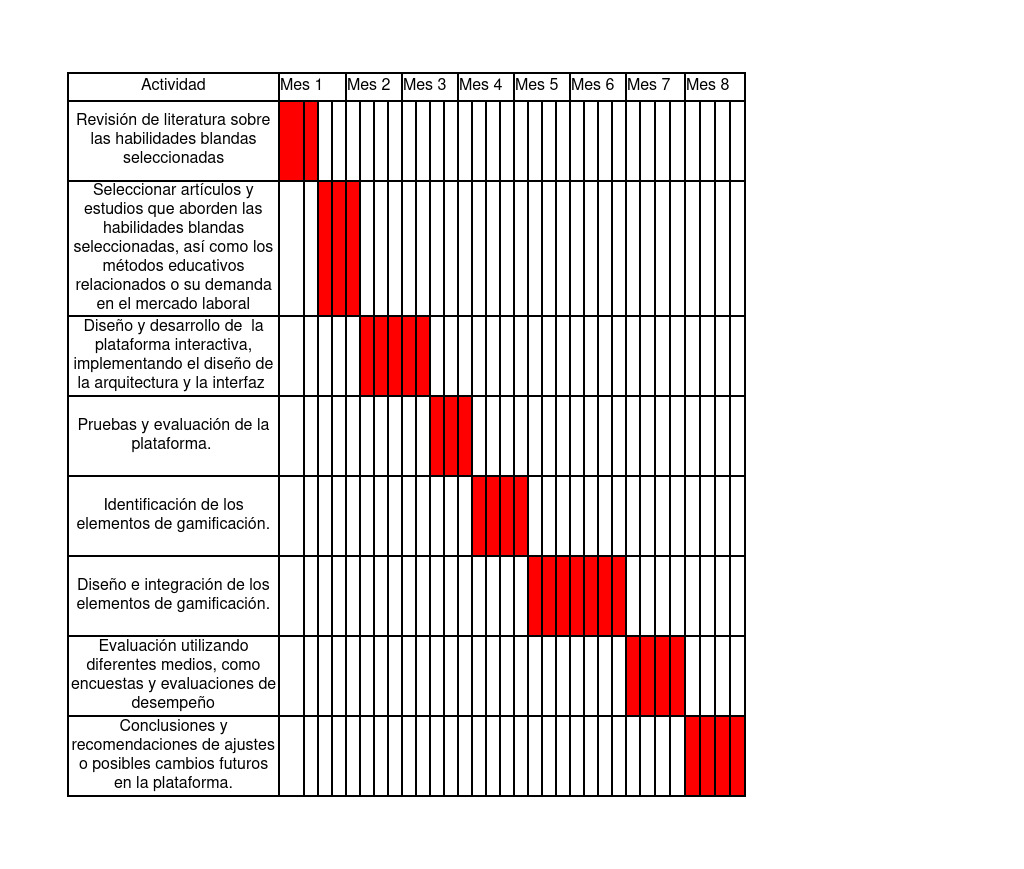
\includegraphics[width=25cm]{Imagenes/tabla-hitos.jpg}
    \caption{Programa de hitos}
\end{figure}